%Thedore Ian Martiny
%Summer 2016 final exam

\documentclass[addpoints,12pt]{exam}
\newcommand{\naturals}{\mathbb{N}}
\newcommand{\integers}{\mathbb{Z}}
\newcommand{\reals}{\mathbb{R}}
\renewcommand{\baselinestretch}{1.5}
%\setlength{\textwidth}{16cm}
\usepackage{amsfonts}
\usepackage{amsmath}
\usepackage{amsthm}
\usepackage{amssymb}
\usepackage{color}
\usepackage{colortbl}
\usepackage{fullpage}
\usepackage{graphicx}
\usepackage[utf8]{inputenc}
\usepackage{listings}
\usepackage{multicol}
\usepackage{nopageno}
\usepackage{setspace}
\usepackage{wasysym}
\usepackage{xcolor}
 
\definecolor{codegreen}{rgb}{0,0.6,0}
\definecolor{codegray}{rgb}{0.5,0.5,0.5}
\definecolor{codepurple}{rgb}{0.58,0,0.82}
\definecolor{backcolour}{rgb}{0.95,0.95,0.92}
\definecolor{Gray}{gray}{0.85}
 
\lstdefinestyle{mystyle}{
    backgroundcolor=\color{backcolour},   
    commentstyle=\color{codegreen},
    keywordstyle=\color{magenta},
    numberstyle=\tiny\color{codegray},
    stringstyle=\color{codepurple},
    basicstyle=\footnotesize,
    breakatwhitespace=false,         
    breaklines=true,                 
    captionpos=b,                    
    keepspaces=true,                 
    numbers=left,                    
    numbersep=5pt,                  
    showspaces=false,                
    showstringspaces=false,
    showtabs=false,                  
    tabsize=2
}
\newcolumntype{a}{>{\columncolor{Gray}}c} 
\lstset{style=mystyle}
\begin{document}
\singlespacing
\hspace*{\fill}\textbf{Name:}\underline{\hspace{8cm}}

\begin{center}
  {\large\textbf{CSCI 2824 - Discrete Structures}}

  {\large\textbf{Final Exam - Part 1}}
\end{center}

Grade: \underline{\hspace{1cm}} /\numpoints
%Grade: \numpoints /\numpoints


\begin{questions}
  \question[12] Add the following numbers without converting to base-10.
  \begin{parts}
    \part $1101_2 + 101100_2 + 110110101_2$
    \vspace*{5cm}
    \begin{solution}
    \end{solution}

    \part \texttt{0x}$A03_{16} + \texttt{0x}4B07A_{16}$
    \vspace*{5cm}
    \begin{solution}
    \end{solution}

    \part $\texttt{0x}1E9_{16} + 1101101_2$
    \vspace*{5cm}
    \begin{solution}
    \end{solution}
  \end{parts}

  \newpage
  \question[12] Decompose the following function
  \begin{parts}
    \part Into three functions, $f,g,h$ such that the given function is $f\circ g\circ h$.
    \[
      \log_2 (x^2 +2)
    \]
    \vspace*{4cm}
    \begin{solution}
    \end{solution}

    \part Into three functions $f,g,h$ such that the given function is $f\circ g\circ h$.
    \[
      \left( 3 + \sin(x) \right)^4
    \]
    \vspace*{4cm}
    \begin{solution}
      $\reals$
    \end{solution}

    \part Into four function $f,g,h,j$ such that the given function is $f\circ g\circ h\circ j$.
    \[
      \frac{1}{(\cos(6x))^3}
    \]
    \vspace*{4cm}
    \begin{solution}
    \end{solution}
  \end{parts}

  \newpage
  \question[20] Determine whether the following are equivalence relations on the set of all people.
  \begin{parts}
    \part For people $x,y$, $(x,y)\in R$ if $x$ and $y$ have the same height.
    \vspace*{8cm}
    \begin{solution}
    \end{solution}

    \part For people $x,y$, $(x,y) \in R$ if $x$ and $y$ have at some time lived in the same country.
    \vspace*{4cm}
    \begin{solution}
    \end{solution}
  \end{parts}

  \newpage
  \question[26] For the following questions, consider the numbers 5 through 200 inclusive.
  \begin{parts}
    \part How many numbers consist of distinct digits? (123 consists of distinct digits, whereas 11 does not)
    \vspace*{8cm}
    \begin{solution}
    \end{solution}

    \part How many do not contain the digit 0?
    \vspace*{6cm}
    \begin{solution}
    \end{solution}
  \end{parts}

  \newpage
  \question[30] Find an Euler tour for this graph:
  \begin{center}
    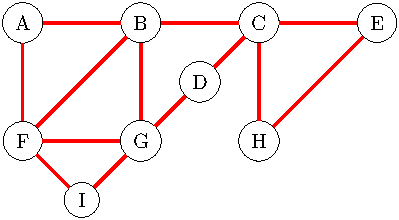
\includegraphics{euler.pdf}
  \end{center}
  You may write your solution either as a sequence of nodes or REDRAW the graph with numbered edges to indicate order.
  \vspace*{10cm}
  \begin{solution}
  \end{solution}
\end{questions}
\end{document}
